\documentclass[11pt]{article}
\usepackage{inputenc,hyperref,a4wide,color,boxedminipage,Sweave,listings}

%\usepackage{Sweave,hyperref}

%\VignetteIndexEntry{HTMLreport}
%\VignettePackage{doBy}

\title{The \texttt{Rmarkup()} function in the \texttt{doBy} package}
\author{S{\o}ren H{\o}jsgaard}

\begin{document}

\bibliographystyle{dcu}
\maketitle
\tableofcontents


\renewenvironment{Schunk}{\begin{center}
    \scriptsize
    \begin{boxedminipage}{0.95\textwidth}}{
    \end{boxedminipage}\end{center}}

\def\proglang#1{{#1}}
\def\pkg#1{{\bf #1}}
\def\doby{\pkg{doBy}}
\def\code#1{\texttt{#1}}
\def\shd#1{\footnote{SHD: #1}}
\def\rep{\code{Rmarkup()}}
\def\R{\proglang{R}}



\parindent0pt\parskip5pt

\section{Introduction}
\label{sec:introduction}

The \rep\ function in the \doby\ package provides facilities for
making reproducible statistical analyses. \rep\ translates an
\R--script (a file with \R\ commands and text comments) into an HTML
document. This HTML document contains the text (possibly with some
markup) and the \R--code along with the results from executing the
\R--code (i.e.\ tables, graphics etc). Section~\ref{sec:introexample}
shows an example of what \rep\ does.

Reproducible analysis for \R\ combined with \LaTeX\ is facilitated by
the Sweave system, \cite{Sweave}. The \pkg{odfweave} package for \R,
\cite{odfWeave} provides similar facilities for using R in conjunction
with the text format OpenDocumentText (as used in the OpenOffice
program suite).  \rep\ is patterned after \code{Sweave}, see also
\url{http://www.stat.uni-muenchen.de/~leisch/Sweave/Sweave-manual.pdf}. In
particular, specification of \R--code follows the \code{noweb} syntax
also employed by Sweave. \rep\ allows some markup facilities for the
text. These are inspired by \code{txt2tags} markups (see
\url{http://txt2tags.org/}). (Details are provided in
Section~\ref{sec:markup}). \rep\ is implemented by using the
\code{RweaveHTML} driver in the \pkg{R2HTML}, \cite{R2HTML}.


\section{Introductory example}
\label{sec:introexample}

A small example is shown in Figure~\ref{fig:src1}. This \R--script
contains \R\ code and text comments (in the lines starting with
\code{\#\#}).



\begin{figure}[ht]
  \centering
  \fbox{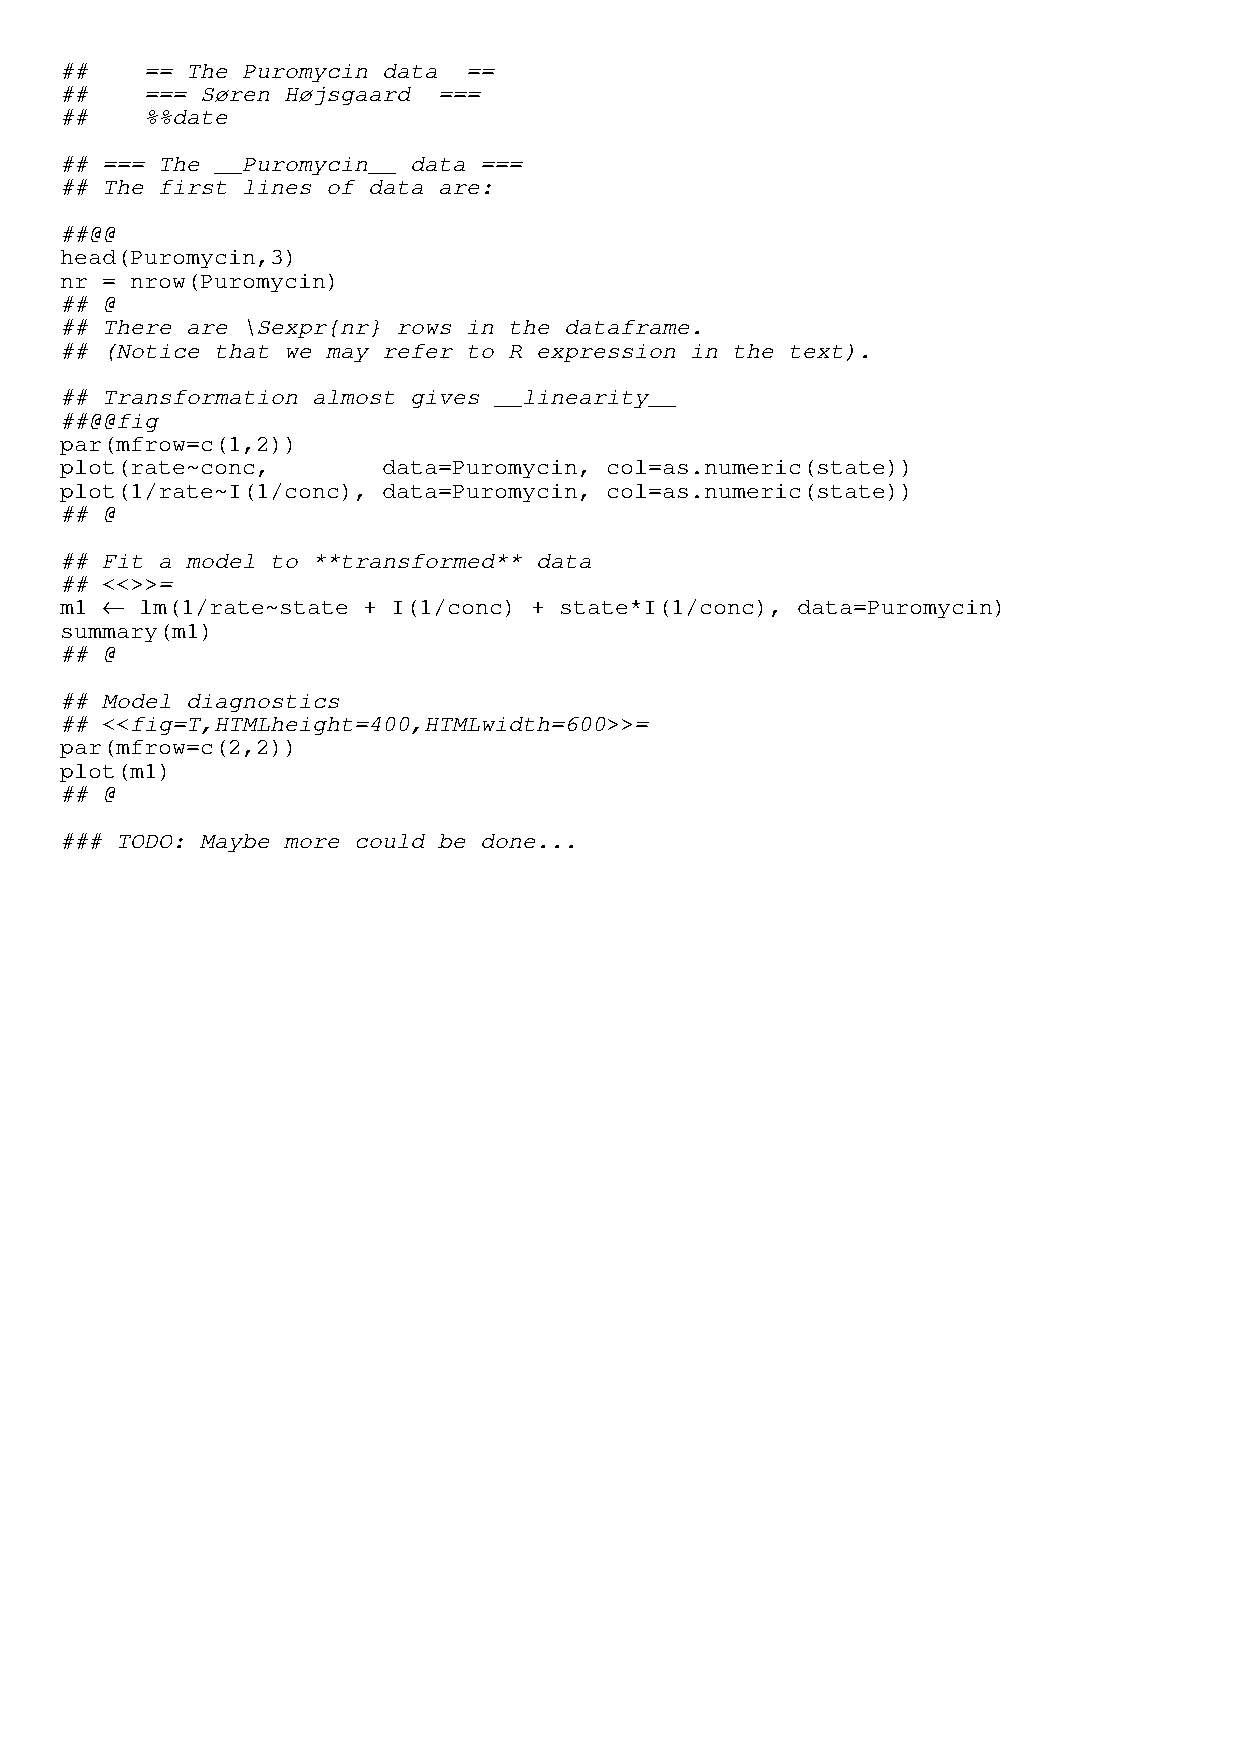
\includegraphics[page=1]{Ex1Puro.pdf}}
  \caption{An \R--script file with a few markups of text.}
  \label{fig:src1}
\end{figure}

This script is processed with
\begin{Schunk}
\begin{Sinput}
 library(doBy)
 Rmarkup("Ex1Puro.R")
\end{Sinput}
\end{Schunk}
and the result is an
HTML document which is shown in Figures~\ref{fig:res1}, \ref{fig:res2}
and \ref{fig:res3}.



\begin{figure}[ht]
  \centering
  \fbox{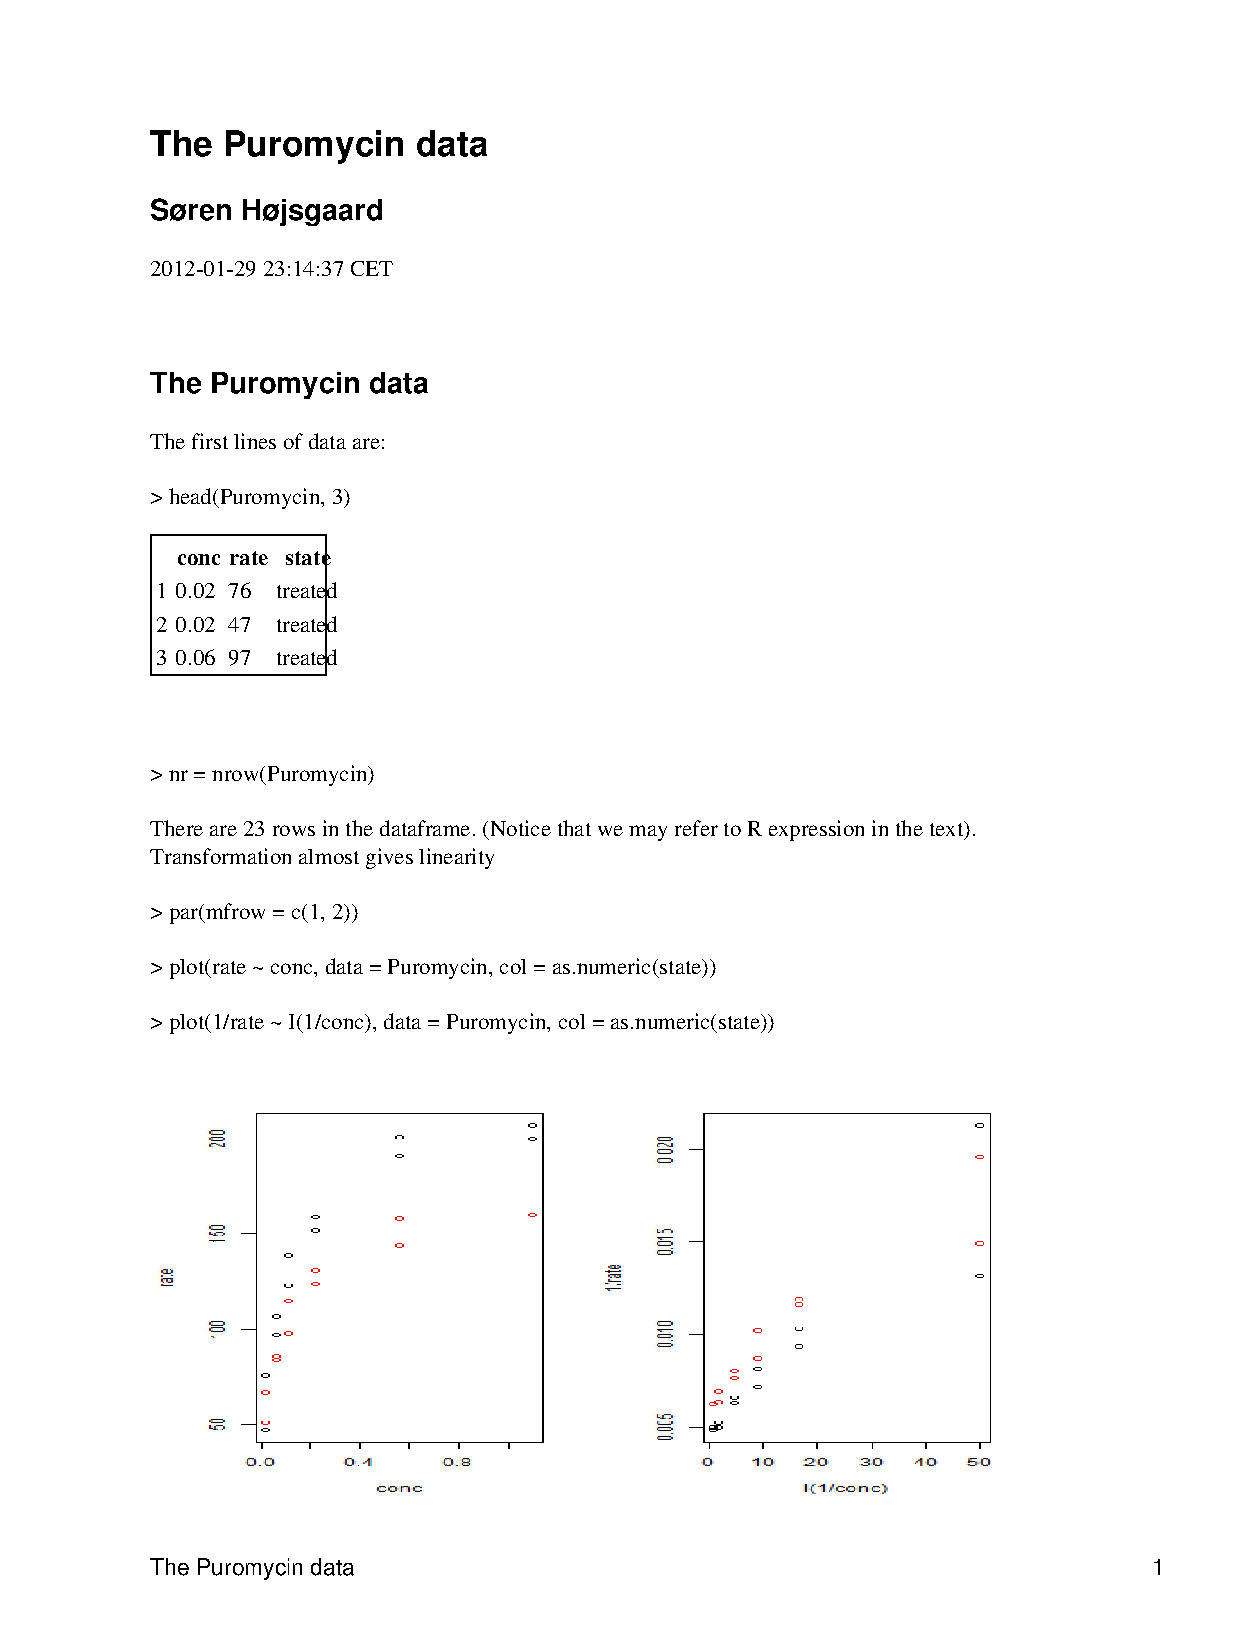
\includegraphics[page=1]{Ex1Puro-REPORT.pdf}}
  \caption{The resulting HTML document produced by \rep.}
  \label{fig:res1}
\end{figure}

\begin{figure}[ht]
  \centering
  \fbox{\includegraphics[page=2]{Ex1Puro-REPORT.pdf}}
  \caption{The resulting HTML document produced by \rep.}
  \label{fig:res2}
\end{figure}

\begin{figure}[ht]
  \centering
  \fbox{\includegraphics[page=3]{Ex1Puro-REPORT.pdf}}
  \caption{The resulting HTML document produced by \rep.}
  \label{fig:res3}
\end{figure}



% See also
% \url{http://cran.r-project.org/web/packages/doBy/index.html}
% for the HTML version of the document.



\section{Markup of R-script}
\label{sec:markup}

All text lines start with one or more hashes (\code{\#}) because these
lines are to be regarded as comments by \R.

\begin{itemize}
\item A line starting with one or two hashes is regarded as a text which
  is transferred (possibly after some additional processing; see below)
  to the resulting HTML document.
\item A line starting with three hashes is not transferred to the HTML
  document. (This is useful e.g. for TODOs).
\end{itemize}

\subsection{Headings and text beautifiers}
\label{sec:xxx}

\begin{itemize}
\item Headings at different font
  sizes are produced with (there can be 6 levels of headings):

  \verb'= Title level 1 =', \verb'== Title level 2 ==',
  \verb'=== Title level 3 ==='


\item The time of creation of the HTML document is produced by

  \verb'%%date'.

\item{Beautifiers:
    {\bf boldface},
    {\it italics},
    \underline{underline},
    \code{monospace}
    :}
  These are produced with:

  \verb'**'boldface\verb'**',  \verb'//'italics\verb'//'
  \verb'__'underline\verb'__', \verb'&&'monospace\verb'&&'

\item The beautifiers can be combined in any way, e.g.

  \verb'**__'some text\verb'__**'.

\item The text beautifiers can be used in the headings.

\end{itemize}

\subsection{Markups must appear on one line}
\label{sec:xxx}

\begin{itemize}
\item All text markups must appear on one line. For example, the
  following will produce a heading in a large font,
\begin{verbatim}
## = HERE COMES A TITLE =
\end{verbatim}
whereas a heading in a large font will not be produced if one writes e.g.
\begin{verbatim}
## =
##   HERE COMES A TITLE
## =
\end{verbatim}

\end{itemize}

\subsection{\R\ code}
\label{sec:xxx}
\begin{itemize}
%
\item A chunk of \R\ code that does not produce graphics:
  The beginning and end of a chunk of \R\ code can be marked with
  \verb'##@@' and \verb'##@'. For example:
\begin{verbatim}
##@@
x <- 1:100
sum(x)
##@
\end{verbatim}
or by using  the noweb syntax
\begin{verbatim}
##<<>>=
x <- 1:100
sum(x)
##@
\end{verbatim}



\item A chunk of \R\ code that does produce graphics:
  The beginning and end of a chunk of \R\ code can be marked with
  \verb'##@@fig' and \verb'##@'. For example:
\begin{verbatim}
##@@fig
x <- 1:100
plot(x)
##@
\end{verbatim}
or by using the noweb syntax
\begin{verbatim}
##<<fig=T>>=
x <- 1:100
plot(x)
##@
\end{verbatim}

\item Notice: Various options may be speficied between  \verb'<<' and
  \verb'>>='; see the example.

\end{itemize}


\section{More advanced use of \rep}
\label{sec:xxx}

It is possible to customize the HTML file by using a css--file. One
may also control the filename for the report. For example
\begin{Schunk}
\begin{Sinput}
 Rmarkup("Ex1Puro.R",cssfile="R2HTML.css", postfix="withCSS")
\end{Sinput}
\end{Schunk}

This creates the file \verb'Ex1Puro-REPORT2.html' which (by
default) is located in the working directory of \R.
The location of the resulting HTML file can be changed by specifying
the \code{destdir}.
The optional \verb'css'--file must
reside in this directory.

\section{Final remarks}
\label{sec:xxx}

A very natural question is why one would possibly use \rep\ when much
more elaborate systems (e.g.\ Sweave and odfWeave) are available:

\begin{itemize}
\item A major advantage of \rep\ is that the input to the function is
  a plain \R\ script file (a text file).
\item A design goal of \rep\ has been that no additional software must be
  installed.
\item There are facilities for marking up text, but these are few and
  easy to remember. However one can always embed standard HTML code in
  the script file for more advanced markups (for example for creating
  lists etc.)
\end{itemize}


\rep\ is based processing the source file line--by--line
(using \verb'gsub()') and therefore all text markups must not be split
over several lines.
The workhorse of \rep\ is the \code{Sweave()} function using the
\code{RweaveHTML} driver of the \code{R2HTML} package.

It is sometimes convenient to convert the HTML report to a pdf file
and this can be done in many ways. A simple way (at least on Windows
platforms) is to use the \code{CutePDF} virtual printer. Another
option is to open the HTML report in \code{OpenOffice} and from there
export the document in pdf format.


% \bibliography{doBy}

\end{document}





% @
% <<echo=T,eval=F>>=
% fname <- "Ex1Puro"

% (sss<-sprintf("a2ps --portrait -1 -B --borders=0 %s.R", fname))
% system(sss)

% (sss<-sprintf("ps2eps -f %s.ps %s.eps", fname, fname))
% system(sss)

% (sss<-sprintf("epstool --copy --bbox %s.eps __tmp__.eps", fname))
% system(sss)

% (sss<-sprintf("epstopdf --outfile=%s.pdf  __tmp__.eps ", fname))
% system(sss)

% @ %def
